\frame{
\frametitle{Navigation: Struktur}
	\begin{figure}
		\centering
		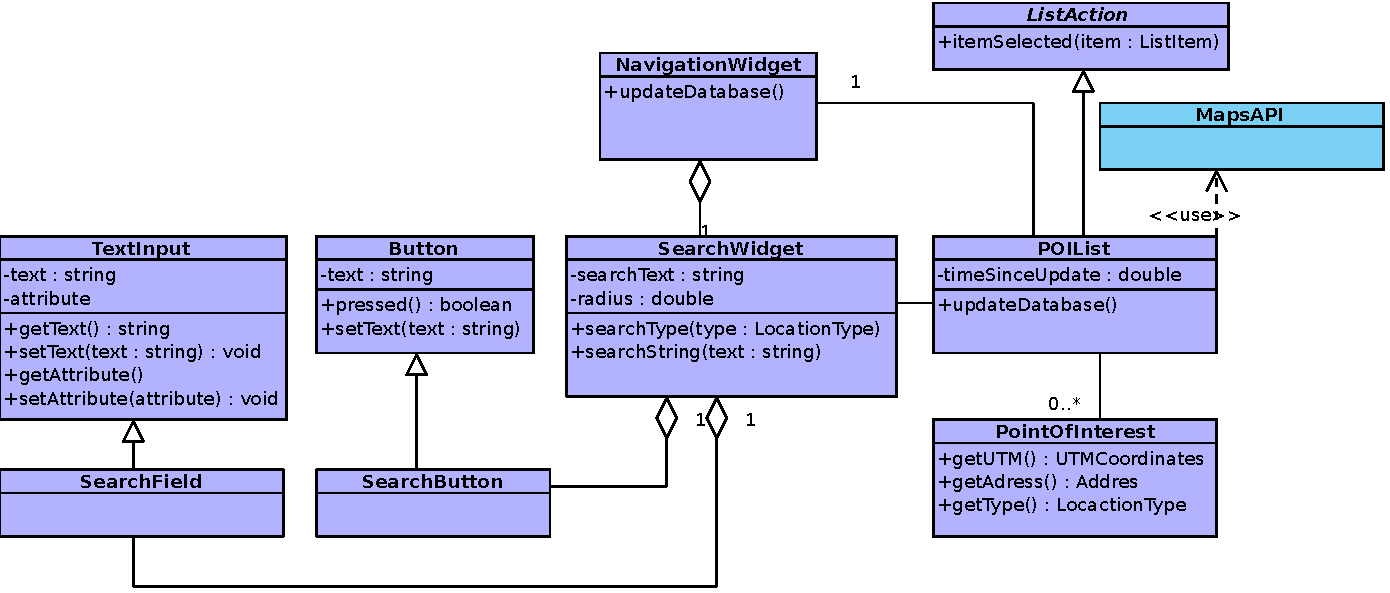
\includegraphics[width=0.9\textwidth]{../grafiken/NavigationW_Class.pdf}	
		\caption{Klassenstruktur für die Navigation.}			
	\end{figure}
}

\frame{
\frametitle{Interessantes}
	\begin{block}{Struktur}
	\begin{itemize}
		\item \textbf{Basisklasse} für interessante Objekte 
		\item \textbf{Addressinformation} für schnelles finden von Orten in der Umgebung
		\item \textbf{UTM-Koordinaten} zur Übergabe an Routenplanner
	\end{itemize}
	\begin{center}
	\begin{figure}
		\centering
		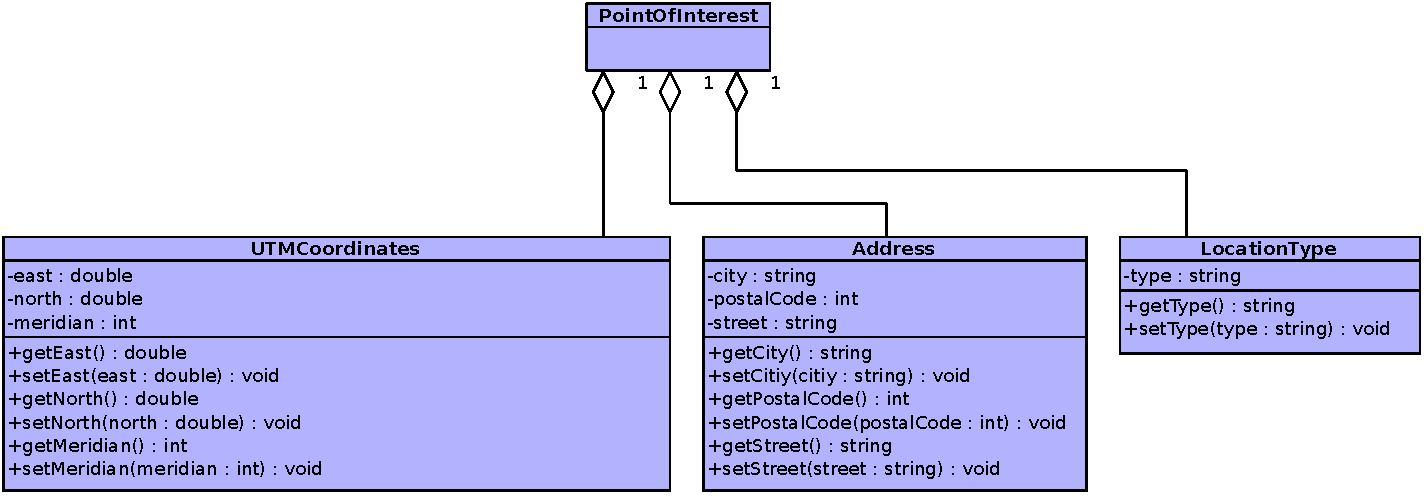
\includegraphics[width=0.7\textwidth]{../grafiken/PointOfInteresst.pdf}
		\caption{Klassenstruktur für interessante Punkte zur Navigation.}
	\end{figure}
	\end{center}
	\end{block}
}
